\documentclass{article}
\usepackage{tikz}
\usetikzlibrary{shapes.geometric, arrows.meta}

\tikzstyle{startstop} = [rectangle, rounded corners, minimum width=3cm, minimum height=1cm,text centered, draw=black, fill=red!30]
\tikzstyle{io} = [trapezium, trapezium left angle=70, trapezium right angle=110, minimum width=3cm, minimum height=1cm, text centered, draw=black, fill=blue!30]
\tikzstyle{process} = [rectangle, minimum width=3cm, minimum height=1cm, text centered, draw=black, fill=orange!30]
\tikzstyle{decision} = [diamond, minimum width=3cm, minimum height=1cm, text centered, draw=black, fill=green!30]
\tikzstyle{arrow} = [thick,->,>=stealth]

\begin{document}

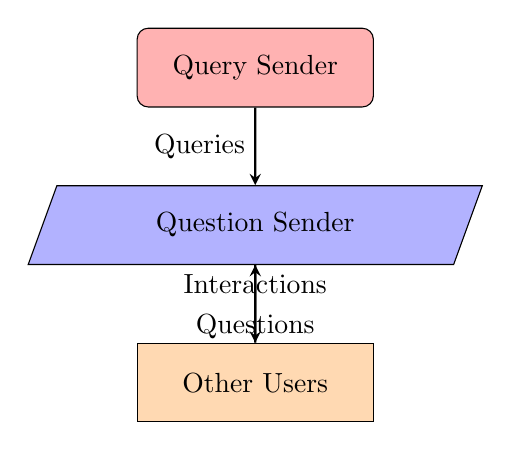
\begin{tikzpicture}[node distance=2cm]

\node (query_sender) [startstop] {Query Sender};
\node (question_sender) [io, below of=query_sender] {Question Sender};
\node (other_users) [process, below of=question_sender] {Other Users};

% Drawing arrows
\draw [arrow] (query_sender) -- node[anchor=east] {Queries} (question_sender);
\draw [arrow] (question_sender) -- node[anchor=north] {Questions} (other_users);
\draw [arrow] (other_users) -- node[anchor=south] {Interactions} (question_sender);

\end{tikzpicture}

\end{document}